
%*****************************************
\chapter{Theoretical Foundation and Hypotheses}\label{ch:third}
%*****************************************


The following chapter presents an unpublished scientific work that will serve as the theoretical core of this thesis. The scientific paper goes by the title 
\begin{center}
 \textit{"Designing Efficient Authentication Mechanisms: There is More to Efficiency than Input Speed."}   
\end{center}
The authors of the paper remain unknown and will, therefore, be referred to as Anonymous et al. \cite{anonymous} in the following course of this thesis. In the first section of this chapter the findings of Anonymous et al. \cite{anonymous} will be presented. In the second section, the limitations of their approach will elaborated and discussed. The last section will illustrate how the author of this thesis intends to validate their findings by reevaluating their approach and proving their hypotheses.

\section{Approach}

As mentioned in Section \ref{2.3}, researchers have tried to detect the factors that most affected the efficiency of smartphone security. They realized that these factors could not be assessed by simply measuring the duration of authentication processes. Also, they discovered a factor that had often been disregarded during the evaluation of efficiency, and that is \textit{orientation time} (see Section \ref{2.2}). The amount preparation and mental effort that is needed to accomplish an authentication task is found to be crucial for user-acceptance \cite{anonymous}. Therefore, new measurement methods are in need which approach the practice of authentication on a human level and which are designed with respect to humans' perception of time and their cognitive abilities. \\

To that, Anonymous et al. \cite{anonymous} made an effort of examining a specific measurement method to better evaluate the usability of authentication mechanisms in terms of their perceived efficiency \cite{anonymous}. They noticed how previous studies indicated that users commonly prefer authentication mechanisms that require little to no mental effort \cite{anonymous, AnatomySmartphone}. So they redefined the architecture of a general authentication process in order to detect the triggers that make authentication exhaustive and inconvenient to users. When found, Anonymous et al. \cite{anonymous} propose that their approach could be considered a prime step towards setting a standard for measuring usability in authentication mechanisms. Moreover, they suggest that their approach could help prevent forming false conclusions regarding the usability aspect of authentication mechanisms when evaluating or comparing them to each other.  \\

\begin{figure}[t!]
\centering
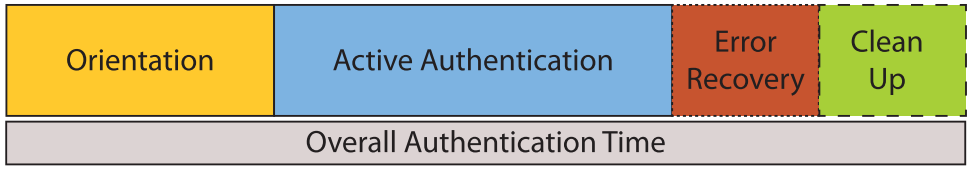
\includegraphics[width=13cm, height=2cm]{Chapters/graphics/Phases.PNG}
\caption{Component phases of an authentication process. While Orientation and Active Authentication (input) phase are the core components of an authentication procedure, Error Recovery may also be included. Clean up phases are not considered part of the authentication process, yet in some designs they are crucial for its completeness \cite{anonymous}. }
\label{fig:phases}
\end{figure}

The following list describes the phases that defince the structure of an authentication process, according to Anonymous et al. \cite{anonymous} (see figure \ref{fig:phases}):

\begin{itemize}
    \item \textbf{\textcolor{orange}{Orientation:}} In previous research, this phase was commonly defined as the \textit{preparation} phase . It defines the period, beginning from the moment when a smartphone screen is switched on, to the moment when the first input action is made . It usually takes place before the user enters their secret. It is the time which they spend either recalling their secret, preparing themselves for its input, or both . Also, it is considered to be the part of the authentication process which requires the most mental effort.  
    \item \textbf{\textcolor{blue}{Active Authentication:}} This phase defines the time a user needs to enter their secret. It begins with the very first input action and ends with the very last\footnote{ \textit{Last input action} means the moment which determines whether unlocking is permitted or denied \cite{anonymous}.}. This phase will be called the \textbf{input} phase, for simplicity reasons.
    \item \textbf{\textcolor{red}{Error Recovery:}} This phase is useful in situations in which an input error occur. Its purpose is to signify to the user that an error had been made. The recovery can take place by requesting a restart of the authentication process, or by allowing so called \textit{undo operations}, which allow the user to correct their mistake and proceed with the input. 
    \item \textbf{\textcolor{green}{Clean Up:}} This phase is not considered to be a solid part of the authentication process, yet in some newly developed mechanisms, it is crucial for completing the authentication. An example for its use, is found in the concepts \textbf{TinyLock} by Kwon et al. \cite{kwon} and \textbf{Whispercore} by Airowaily et al. \cite{Airowaily}. In these designs, the clean up phase is intended to remove oily residues on the smartphone screen and thereby counteracts the chance of potential smudge attacks. 
\end{itemize}

According to Anonymous et al. \cite{anonymous}, \textit{orientation} and \textit{input} phases are considered to be the most essential parts of an authentication process. In previous approaches, the \textit{input} phase has often been considered to define the actual authentication procedure. Consequently, \textit{orientation} time was often disregarded and ignored in usability evaluations. Ananymous et al. \cite{anonymous} describe \textit{error recovery} to be not essentially mandatory for successful authentication, yet very useful for its error management. They also observed that its implementation could have a significant effect on the efficiency of an authentication mechanism. In some cases, its implementation may even trigger the need for further \textit{orientation} or \textit{clean up} phases \cite{anonymous}. This, in return, may cause a longer authentication duration. The implementation of the \textit{clean up} phase depends on the design of the authentication concept. Authentication is possible with or without it (see figure \ref{fig:phases}). \\

By outlining the structure of the authentication process, Anonymous et al. \cite{anonymous} proposed a collection of observations and factors to prove in a user case study. First, they observed that the proportioning of the authentication may phases affects the perceived efficiency of an authentication mechanism. For instance, they noticed that the longer the \textit{orientation} of an authentication mechanism is, the slower and less efficient it is perceived. In fact, cases in which the duration of the \textit{orientation} phase exceeded the \textit{input} phase, have been seen to be widely disliked by users. \\

Second, they noticed that the ordering of the phases might impact perceived efficiency. For instance, \textbf{Pattern Rotation} only consists of two phases, with the \textit{orientation} phase preceding the \textit{input} phase. \textbf{Marbles}, on the other hand, has multiple small \textit{orientation} and \textit{input} phases, ordered in an alternating manner. Anonymous et al. \cite{anonymous} suggested that the latter has the possibility of decreasing the perceived duration of authentication. \\

Third, they suggested that the coherence of the \textit{orientation} and \textit{input} phases also have a potential influence a mechanism's perceived efficiency \cite{anonymous}. Meaning, the less coherent the contexts of \textit{orientation} time and \textit{input} time are, the less efficient and convenient they are perceived. This factor was regarded in the design of \textbf{Marbles} \cite{Marbles}. Thus its tasks alternate between finding the marbles and dragging them into the gap, their contexts complement each other. Through further research Anonymous et al. \cite{anonymous} found that humans tend to perceive periods longer than they are if they consist of many incoherent contexts \cite{anonymous,perception}.\\

Lastly, Anonymous et al. \cite{anonymous} added that \textit{error recovery} should be cautiously managed throughout the authentication process \cite{anonymous}. As mentioned above, the implementation of \textit{error recovery} may result in further \textit{orientation} and \textit{clean up} phases. This observation was shown in findings by Zezschwitz et al. \cite{PatternWild}, discussed in Section \ref{2.2}. They discovered how users tended more towards \textit{pattern} authentication than \textit{pin} because they preferred its management of errors. \textit{Pin} manages the errors through \textit{undo-operations}, which have been shown to be disliked amoungst users. Therefore, they are seldomly used in designs \cite{PatternWild, anonymous}. 

\begin{figure}[t!]
\centering
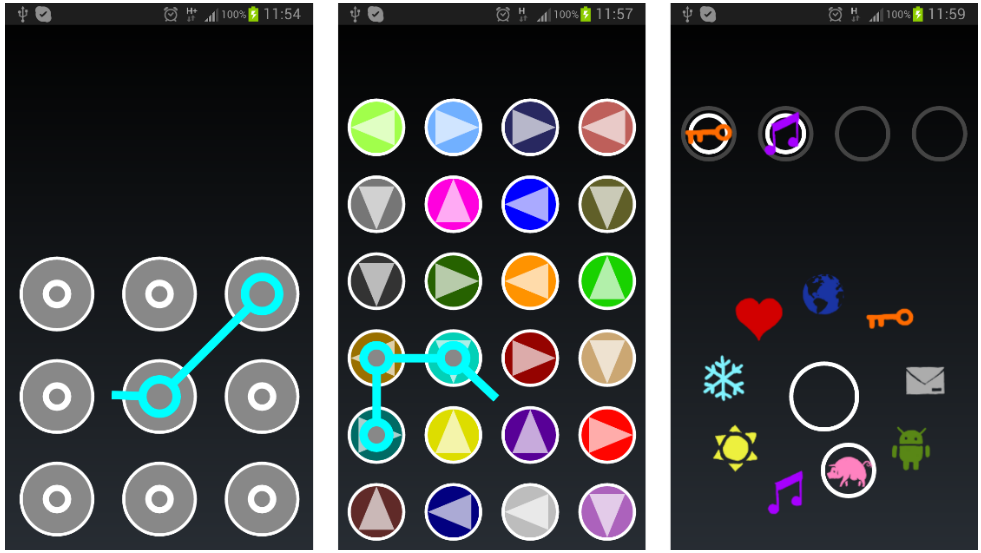
\includegraphics[width=14cm, height=7cm]{Chapters/graphics/androidPatternMarble.PNG}
\caption{The concepts that Anonymous et al. \cite{anonymous} used in their study. Left: Android Unlock Pattern (baseline); Middle: Pattern Rotation; Right: Marbles. Compare with figure \ref{fig:marbles} to see how the concepts were modified in this study \cite{anonymous}.}
\label{fig:android}
\end{figure}

\section{User Case Study}

Anonymous et al. \cite{anonymous} decided to conduct a study in which they mainly focused on the phases, \textit{orientation}, and \textit{input}, as they are the most important phases of an authentication process. To prove their assumptions and observations, they selected three authentication concepts, each representing a different ratio of both phases \cite{anonymous}
\footnote{To better understand the functionalities of the concepts listed above, it is recommended to revisite the approach by Zezschwitz et al. \cite{Marbles}, presented in Section \ref{2.2.3}.}: 

\begin{itemize}
    \item \textbf{Android Unlock Pattern} represented a "\textcolor{red}{short} orientation/\textcolor{red}{short} input" ratio,
    \item \textbf{Pattern Rotation} represented a "\textcolor{blue}{long} orientation/\textcolor{red}{short} input" ratio,
    \item \textbf{Marbles} represented a ratio in which orientation and input time were interlaced.
\end{itemize}

It is important to note that \textit{Pattern Rotation} and \textit{Marbles} \cite{Marbles} were slightly modified in this study. \textit{Pattern Rotation} presented a larger grid than the original design, and in \textit{Marbles}, the elements (marbles) were small images rather than colored dots (see figure \ref{fig:android} and \ref{fig:marbles}). All three concepts were implemented in a prototype which was then installed on the Android smartphones of study participants \cite{anonymous}. The prototype was intended to serve as an authentication system on the participants' phones. Each of the concepts was planned to be tested for ten days \cite{anonymous}. After each ten-day period, an online survey was required to be taken. Also, during the concept-tests, \textit{orientation} and \textit{input} times were logged for each authentication \cite{anonymous}. \textit{Orientation} time was logged from the moment the screen was switched on, to the first input event. \textit{Input} time was logged from the first to the last input event \cite{anonymous}. Participants were allowed to choose their own secrets for the concepts. However, fixed guidelines were set, for instance, patterns for \textit{Android Unlock Pattern} had to consist of six nodes, patterns for \textit{Pattern Rotation} had to consist of five nodes, and secrets in \textit{Marbles} had to consist of four elements \cite{anonymous}.

\subsection{Results}

The study yielded 19 participants and delivered a set of 18 valid data entities \cite{anonymous}. Anonymous et al. \cite{anonymous} were interested in the different outcomes if the took three different approaches to evaluate the efficiency of the three authentication concepts. So, they began with analyzing the overall authentication times of the concepts and noted the following ranking regarding their \textbf{measured performances}\footnote{The concepts are ordered from fastest to slowest (or best to worst) in this and the following rankings of this section.} \cite{anonymous}:

\begin{enumerate}
    \item \textbf{Android Unlock Pattern},
    \item \textbf{Pattern Rotation},
    \item \textbf{Marbles}.
\end{enumerate} 

Then, they only analyzed the measured \textit{input} times of the concepts and  noted the following difference:

\begin{enumerate}
    \item \textbf{Pattern Rotation},
    \item \textbf{Android Unlock Pattern},
    \item \textbf{Marbles}.
\end{enumerate}

Last, they analyzed the measured \textit{orientation} time of the concepts and realized another significantly different outcome. \textit{Android Pattern Unlock} had the shortest \textit{orientation} time of all three concepts, as it required the least amount of mental effort   \cite{anonymous}. Also, \textit{Pattern Rotation} and \textit{Marbles} did not notably differ from each other, in terms of their average \textit{orientation} times \cite{anonymous}. \\


The perceived efficiency of the concepts was rated qualitatively through five-point Likert scales \cite{anonymous}. Results showed that \textit{Android Unlock Pattern} was seen as the fastest of all three concepts. More than half of the participants considered \textit{Marbles} to be efficient, despite it having been measured slower than \textit{Pattern Rotation}. Moreover, half of the participants also perceived \textit{Pattern Rotation} as efficient \cite{anonymous}. Participants were asked if the concepts contented a fast and easy orientation. The results delivered the following ranking \cite{anonymous}: 

\begin{enumerate}
     \item \textbf{Android Unlock Pattern},
    \item \textbf{Marbles},
    \item \textbf{Pattern Rotation}.
\end{enumerate}

Lastly, when asked about the required cognitive effort, all participants approved that Android Pattern Unlock required the least amount of mental effort, followed by Pattern Rotation, then Marbles \cite{anonymous}. \\

\subsection{Design Recommendations}

Based on the results of their study, Anonymous et al. \cite{anonymous} made a list of design recommendations to consider in the creation of authentication concepts. They are intended to optimize the usability of an authentication concept by regulating the following aspects \cite{anonymous}:

\begin{itemize}
    \item \textbf{Recommendation 1:} \textit{"Measure all Stages"}\\
    By including orientation time into time measurements, the possibility of making false conclusions about a concept's usefulness could be prevented.
    \item \textbf{Recommendation 2:} \textit{"Keep Orientation Time Low"}\\
    As Orientation times are disliked by users, it is suggested to keep as short as possible, because the effect of long orientation times cannot counteracted by short input times.
    \item \textbf{Recommendation 3:} \textit{"Optimize the Ratio between Orientation Time and [Input Time]"} \\
    Orientation phases should not be longer than the corresponding input phases, because they not well accepted by users, regardless how fast or efficient a concept's performance is.
    \item \textbf{Recommendation 4:} \textit{"Avoid/Minimize Randomization"}\\ 
    Although randomization is often used as a countermeasure towards attacks (e.g., shoulder surfing), it impacts the perceived efficiency of a concepts negatively and should, therefore, be avoided. Especially in between the tasks of an authentication proecdure.
    \item \textbf{Recommendation 5:} \textit{"Measure Perceived Speed"}\\
    It is recommended that the performance of an authentication concept is not only assessed quantitatively, yet also qualitatively, in order to obtain information how users' perceive certain aspects of the concept (e.g. orientation time).  
    \item \textbf{Recommendation 6:} \textit{"Optimize Context Switches"}\\
    The tasks in an authentication concept should be coherent in terms of their contexts, otherwise they are perceived as usable. 
    \item \textbf{Recommendation 7:} \textit{"Provide Efficient and Non-interrupting Error Recovery"}\\
    Error Recovery should be designed to be as "fast" and simple as possible. A given example for good error recovery is Android Unlock Pattern, as its method is non-disturbing thus errors are indicated through colors.  
    
    
\end{itemize}


\section{Limitations and suggestive improvements} \label{3.3}

This section will first begin by presenting some of the limitations of the study, given by Anonymous et al. \cite{anonymous}. Next, observations on specific qualities of the study will be presented and suggestive improvements on these qualities will be discussed. 

According to Anonymous et al. \cite{anonymous}, the overall perception of the tested concepts could have been influenced by the participants' general preference \cite{anonymous} because a person's culture and history have shown to influence their acceptance of a particular system \cite{Harbach:2016} (Section \ref{2.2.1}). The complementary study, presented in Chapter \ref{ch:fifth} is intended to exclude this limitation by developing a prototype in which particular ratios are represented through the same concept. That way, a more genuine evaluation of the ratios would be possible, without any interference of participants' preferences regarding a particular concept. Moreover, Anonymous et al. \cite{anonymous} stated that the measured times for \textit{orientation} might have differed from the actual times \cite{anonymous}. Reason being that the measurements for the \textit{orientation} times began as soon as the smartphone screen was turned on. However, not every screen activation was always immediately followed by an authentication \cite{anonymous}. A possible solution for rectifying this inaccuracy, is to isolate the \textit{orientation} phase from any other possible action. The concept for the complementary study will be designed in a way that requires the user to actively initiate the authentication process. That way, a fix and accurate starting point for the \textit{orientation} time can be defined.\\

Further limitations, observed by the author of this thesis are the following: The ratios chosen by Anonymous et al. \cite{anonymous} might not have been suitable enough to receive a definite result on whether users truly prefer short \textit{orientation time} over long \textit{orientation time}. It would be interesting to observe the outcome of testing ratios that have the same temporal arrangement, yet are contrasting regarding the lengths of their phases. Thus not included by Anonymous et al., it is considered to include the ratio \textit{"short orientation/long input"} into our the complementary study. The author suggests that by mainly focusing on the ratios \textit{"long orientation/short input"} and \textit{"short orientation/long input"}, and by setting the ratio \textit{"short orientation/short input"} as a baseline, one could receive more detailed results on users' attitude towards authentication concepts with different lengths of \textit{orientation} phases. A further suggestion is to observe whether different lengths of \textit{input} phases might play a role in users' preference and perception of efficiency. Lastly, it is suggested that by allowing study participants to qualitatively evaluate the ratios in comparison to each other, one could receive more detailed and precise information about which ratio is generally perceived as efficient and which is not. \\

The next chapter of this thesis will present an interaction system which was specifically designed for the sake of the complementary study, later presented in Chapter \ref{ch:fifth}. It was created to implement a specially designed concept, intended to represent each of the previously mentioned ratios. Its sole purpose was to serve as  supportive feature of the study and no further. Nonetheless it is important, for the scope of this thesis, to understand the design choices and the thought processes that were involved in creating this system, as they were made from a user-centered design approach and also included HCI principles, to assure the creation of a system that is suitable for the intentions and desired goals of the study. 







